\documentclass{beamer}
\usepackage[spanish]{babel}
\usepackage[backend=biber, style=authoryear-icomp]{biblatex}
\resetcounteronoverlays{exx}
\usepackage{mdframed}
\usepackage{tikz}
% tikzlibrary.code.tex
%
% Copyright 2010-2011 by Laura Dietz
% Copyright 2012 by Jaakko Luttinen
%
% This file may be distributed and/or modified
%
% 1. under the LaTeX Project Public License and/or
% 2. under the GNU General Public License.
%
% See the files LICENSE_LPPL and LICENSE_GPL for more details.

% Load other libraries

%\newcommand{\vast}{\bBigg@{2.5}}
% newcommand{\Vast}{\bBigg@{14.5}}
% \usepackage{helvet}
% \renewcommand{\familydefault}{\sfdefault}

\usetikzlibrary{shapes}
\usetikzlibrary{fit}
\usetikzlibrary{chains}
\usetikzlibrary{arrows}

% Latent node
\tikzstyle{latent} = [circle,fill=white,draw=black,inner sep=1pt,
minimum size=20pt, font=\fontsize{10}{10}\selectfont, node distance=1]
% Observed node
\tikzstyle{obs} = [latent,fill=gray!25]
% Invisible node
\tikzstyle{invisible} = [latent,minimum size=0pt,color=white, opacity=0, node distance=0]
% Constant node
\tikzstyle{const} = [rectangle, inner sep=0pt, node distance=0.1]
%state
\tikzstyle{estado} = [latent,minimum size=8pt,node distance=0.4]
%action
\tikzstyle{accion} =[latent,circle,minimum size=5pt,fill=black,node distance=0.4]
\tikzstyle{fijo} =[latent,circle,minimum size=5pt,fill=black]


% Factor node
\tikzstyle{factor} = [rectangle, fill=black,minimum size=10pt, draw=black, inner
sep=0pt, node distance=1]
% Deterministic node
\tikzstyle{det} = [latent, rectangle]

% Plate node
\tikzstyle{plate} = [draw, rectangle, rounded corners, fit=#1]
% Invisible wrapper node
\tikzstyle{wrap} = [inner sep=0pt, fit=#1]
% Gate
\tikzstyle{gate} = [draw, rectangle, dashed, fit=#1]

% Caption node
\tikzstyle{caption} = [font=\footnotesize, node distance=0] %
\tikzstyle{plate caption} = [caption, node distance=0, inner sep=0pt,
below left=5pt and 0pt of #1.south east] %
\tikzstyle{factor caption} = [caption] %
\tikzstyle{every label} += [caption] %

\tikzset{>={triangle 45}}

%\pgfdeclarelayer{b}
%\pgfdeclarelayer{f}
%\pgfsetlayers{b,main,f}

% \factoredge [options] {inputs} {factors} {outputs}
\newcommand{\factoredge}[4][]{ %
  % Connect all nodes #2 to all nodes #4 via all factors #3.
  \foreach \f in {#3} { %
    \foreach \x in {#2} { %
      \path (\x) edge[-,#1] (\f) ; %
      %\draw[-,#1] (\x) edge[-] (\f) ; %
    } ;
    \foreach \y in {#4} { %
      \path (\f) edge[->,#1] (\y) ; %
      %\draw[->,#1] (\f) -- (\y) ; %
    } ;
  } ;
}

% \edge [options] {inputs} {outputs}
\newcommand{\edge}[3][]{ %
  % Connect all nodes #2 to all nodes #3.
  \foreach \x in {#2} { %
    \foreach \y in {#3} { %
      \path (\x) edge [->,#1] (\y) ;%
      %\draw[->,#1] (\x) -- (\y) ;%
    } ;
  } ;
}

% \factor [options] {name} {caption} {inputs} {outputs}
\newcommand{\factor}[5][]{ %
  % Draw the factor node. Use alias to allow empty names.
  \node[factor, label={[name=#2-caption]#3}, name=#2, #1,
  alias=#2-alias] {} ; %
  % Connect all inputs to outputs via this factor
  \factoredge {#4} {#2-alias} {#5} ; %
}

% \plate [options] {name} {fitlist} {caption}
\newcommand{\plate}[4][]{ %
  \node[wrap=#3] (#2-wrap) {}; %
  \node[plate caption=#2-wrap] (#2-caption) {#4}; %
  \node[plate=(#2-wrap)(#2-caption), #1] (#2) {}; %
}

% \gate [options] {name} {fitlist} {inputs}
\newcommand{\gate}[4][]{ %
  \node[gate=#3, name=#2, #1, alias=#2-alias] {}; %
  \foreach \x in {#4} { %
    \draw [-*,thick] (\x) -- (#2-alias); %
  } ;%
}

% \vgate {name} {fitlist-left} {caption-left} {fitlist-right}
% {caption-right} {inputs}
\newcommand{\vgate}[6]{ %
  % Wrap the left and right parts
  \node[wrap=#2] (#1-left) {}; %
  \node[wrap=#4] (#1-right) {}; %
  % Draw the gate
  \node[gate=(#1-left)(#1-right)] (#1) {}; %
  % Add captions
  \node[caption, below left=of #1.north ] (#1-left-caption)
  {#3}; %
  \node[caption, below right=of #1.north ] (#1-right-caption)
  {#5}; %
  % Draw middle separation
  \draw [-, dashed] (#1.north) -- (#1.south); %
  % Draw inputs
  \foreach \x in {#6} { %
    \draw [-*,thick] (\x) -- (#1); %
  } ;%
}

% \hgate {name} {fitlist-top} {caption-top} {fitlist-bottom}
% {caption-bottom} {inputs}
\newcommand{\hgate}[6]{ %
  % Wrap the left and right parts
  \node[wrap=#2] (#1-top) {}; %
  \node[wrap=#4] (#1-bottom) {}; %
  % Draw the gate
  \node[gate=(#1-top)(#1-bottom)] (#1) {}; %
  % Add captions
  \node[caption, above right=of #1.west ] (#1-top-caption)
  {#3}; %
  \node[caption, below right=of #1.west ] (#1-bottom-caption)
  {#5}; %
  % Draw middle separation
  \draw [-, dashed] (#1.west) -- (#1.east); %
  % Draw inputs
  \foreach \x in {#6} { %
    \draw [-*,thick] (\x) -- (#1); %
  } ;%
}


\usepackage{blindtext}
\usepackage{tipa}
\usepackage{cgloss4e}
\usepackage{gb4e}
\usepackage{qtree}
\usepackage{enumerate}
\usepackage{longtable}
\graphicspath{ {../img/} } % declaramos donde estan las imagenes
\usepackage[labelformat=simple]{subcaption} % para varias imagenes juntas
\renewcommand\thesubfigure{(\alph{subfigure})}
\usepackage[utf8]{inputenc}
\usepackage{amsmath}
\usepackage{amsfonts} % simbolos como el I de matriz identidad
\usepackage{graphicx} % paquete para ver imagenes
\usepackage{setspace}
\usepackage[T1]{fontenc}
\usepackage{parskip}
\usepackage{color}
\usetheme{Copenhagen}
\definecolor{frenchblue}{rgb}{0.0, 0.45, 0.73} % ESTE!!!!
\definecolor{myblue1}{RGB}{35,119,189}
\definecolor{myblue2}{RGB}{95,179,238}
\definecolor{myblue3}{RGB}{129,168,207}
\definecolor{myblue4}{RGB}{26,89,142}

\setbeamercolor{block body}{bg=frenchblue!50}
\setbeamercolor*{structure}{fg=frenchblue,bg=blue}
\setbeamertemplate{frametitle}[default][center]
\setlength{\parskip}{12pt}
\useoutertheme{infolines} % me comia mucho espacio de la otra fgorma
\makeatother
\setbeamertemplate{footline}
{
  \leavevmode%
  \hbox{%
  \begin{beamercolorbox}[wd=.3\paperwidth,ht=2.25ex,dp=1ex,center]{author in head/foot}%
    \usebeamerfont{author in head/foot}\insertshortauthor
  \end{beamercolorbox}%
  \begin{beamercolorbox}[wd=.6\paperwidth,ht=2.25ex,dp=1ex,center]{title in head/foot}%
    \usebeamerfont{title in head/foot}\insertshorttitle
  \end{beamercolorbox}%
  \begin{beamercolorbox}[wd=.1\paperwidth,ht=2.25ex,dp=1ex,center]{date in head/foot}%
    \insertframenumber{} / \inserttotalframenumber\hspace*{1ex}
  \end{beamercolorbox}}%
  \vskip0pt%
}
\makeatletter
\setbeamertemplate{navigation symbols}{}
%\setbeameroption{show notes}   
\setbeameroption{hide notes}



\title[Estimación de habilidad y la asignación de handicap]{Estimación de habilidad y la asignación de handicap. Aplicación al juego de go}
\author[Matias Mazzanti]{Matias Mazzanti\\ \footnotesize Director: Dr. Esteban Mocskos\\ \footnotesize Co-Director: Dr. Pablo Balenzuela}


\institute{Universidad de Buenos Aires}
%\logo{\includegraphics[height=2.5cm]{../df.jpg}}
\titlegraphic{ \includegraphics[,height=1.3cm,keepaspectratio]{../licar.png}
       ~\hspace{3cm}
       \includegraphics[height=1.8cm,keepaspectratio]{../df.jpg}
     }
\begin{document}

\begin{frame}

\maketitle

\end{frame}
%%%%%%%%%%%%%%%%%%%%%%%%%%%%%%%%%%%%%%%%%%%%%%%%%%%%%%%%%%%%%%%%%%%%%%%%%%%%%%%%%%%%%%%%%%%%%%%%%%%%



\begin{frame}
\frametitle{Motivacion}

\begin{itemize}
 \item Establecimiento de rankings: Sistemas educativos, deportes e industria de los videojuegos
 \item Habilidad: eficiencia de un agente, variable oculta
 \item Sistema de ventajas: handicap, partidas desafiantes (equiprobables)
 \item Modelos: TrueSkill, bayesiano, grafico de factores
 \item Problema: mejorar sistema de ranking y la asignacion de los valores de handicap
 \item Propuesta: modelar las piedras de handicap en el juego go utilizando TrueSkill
\end{itemize}

% queda descolgado todo... es muy dificil explicar todas las cosas en una slide, quizas ir aun mas generico


% \note{
% this is a note (does not understand markdown and
% and wont work in other outputs formats (such 
% as ioslides or Slidy
% }
\end{frame}
%%%%%%%%%%%%%%%%%%%%%%%%%%%%%%%%%%%%%%%%%%%%%%%%%%%%%%%%%%%%%%%%%%%%%%%%%%%%%%%%%%%%%%%%%%%%%%%%%%%%

\begin{frame}
\frametitle{Organizacion}
\begin{columns}
 \column{.3\textwidth}

\column{.7\textwidth}
\begin{itemize}
\setlength\itemsep{0.5cm}
 \item Introduccion
 \item Metodos
 \item Validacion
 \item Resultados
 \item Conclusiones 
\end{itemize}
\end{columns}
\end{frame}
%%%%%%%%%%%%%%%%%%%%%%%%%%%%%%%%%%%%%%%%%%%%%%%%%%%%%%%%%%%%%%%%%%%%%%%%%%%%%%%%%%%%%%%%%%%%%%%%%%%%
\section{Introduccion}
\begin{frame}
\frametitle{Go}

\begin{columns}
 \column{.7\textwidth}
 
\begin{itemize}
 \item Juego de mesa 1 vs 1, fichas negras vs blancas
 \item Ficha negra inicializa el juego (jugador mas debil)
 \item Tableros: 9x9, 13x13, 19x19, otros
 \item Movimiento: 1 ficha por turno de forma alternada, fichas en intersecciones del grillado, fichas inmoviles por el resto de la partida
 \item Objetivo: Sumar puntos formando territorios y caputrando fichas enemigas
 \item Finalizacion: Abandono, por tiempo, por puntos
 \item Reglas sencillas con gran diversidad de jugadas posibles teniendo asi gran complejidad
\end{itemize}

\column{.3\textwidth}
  \begin{figure}[H]
	\centering
	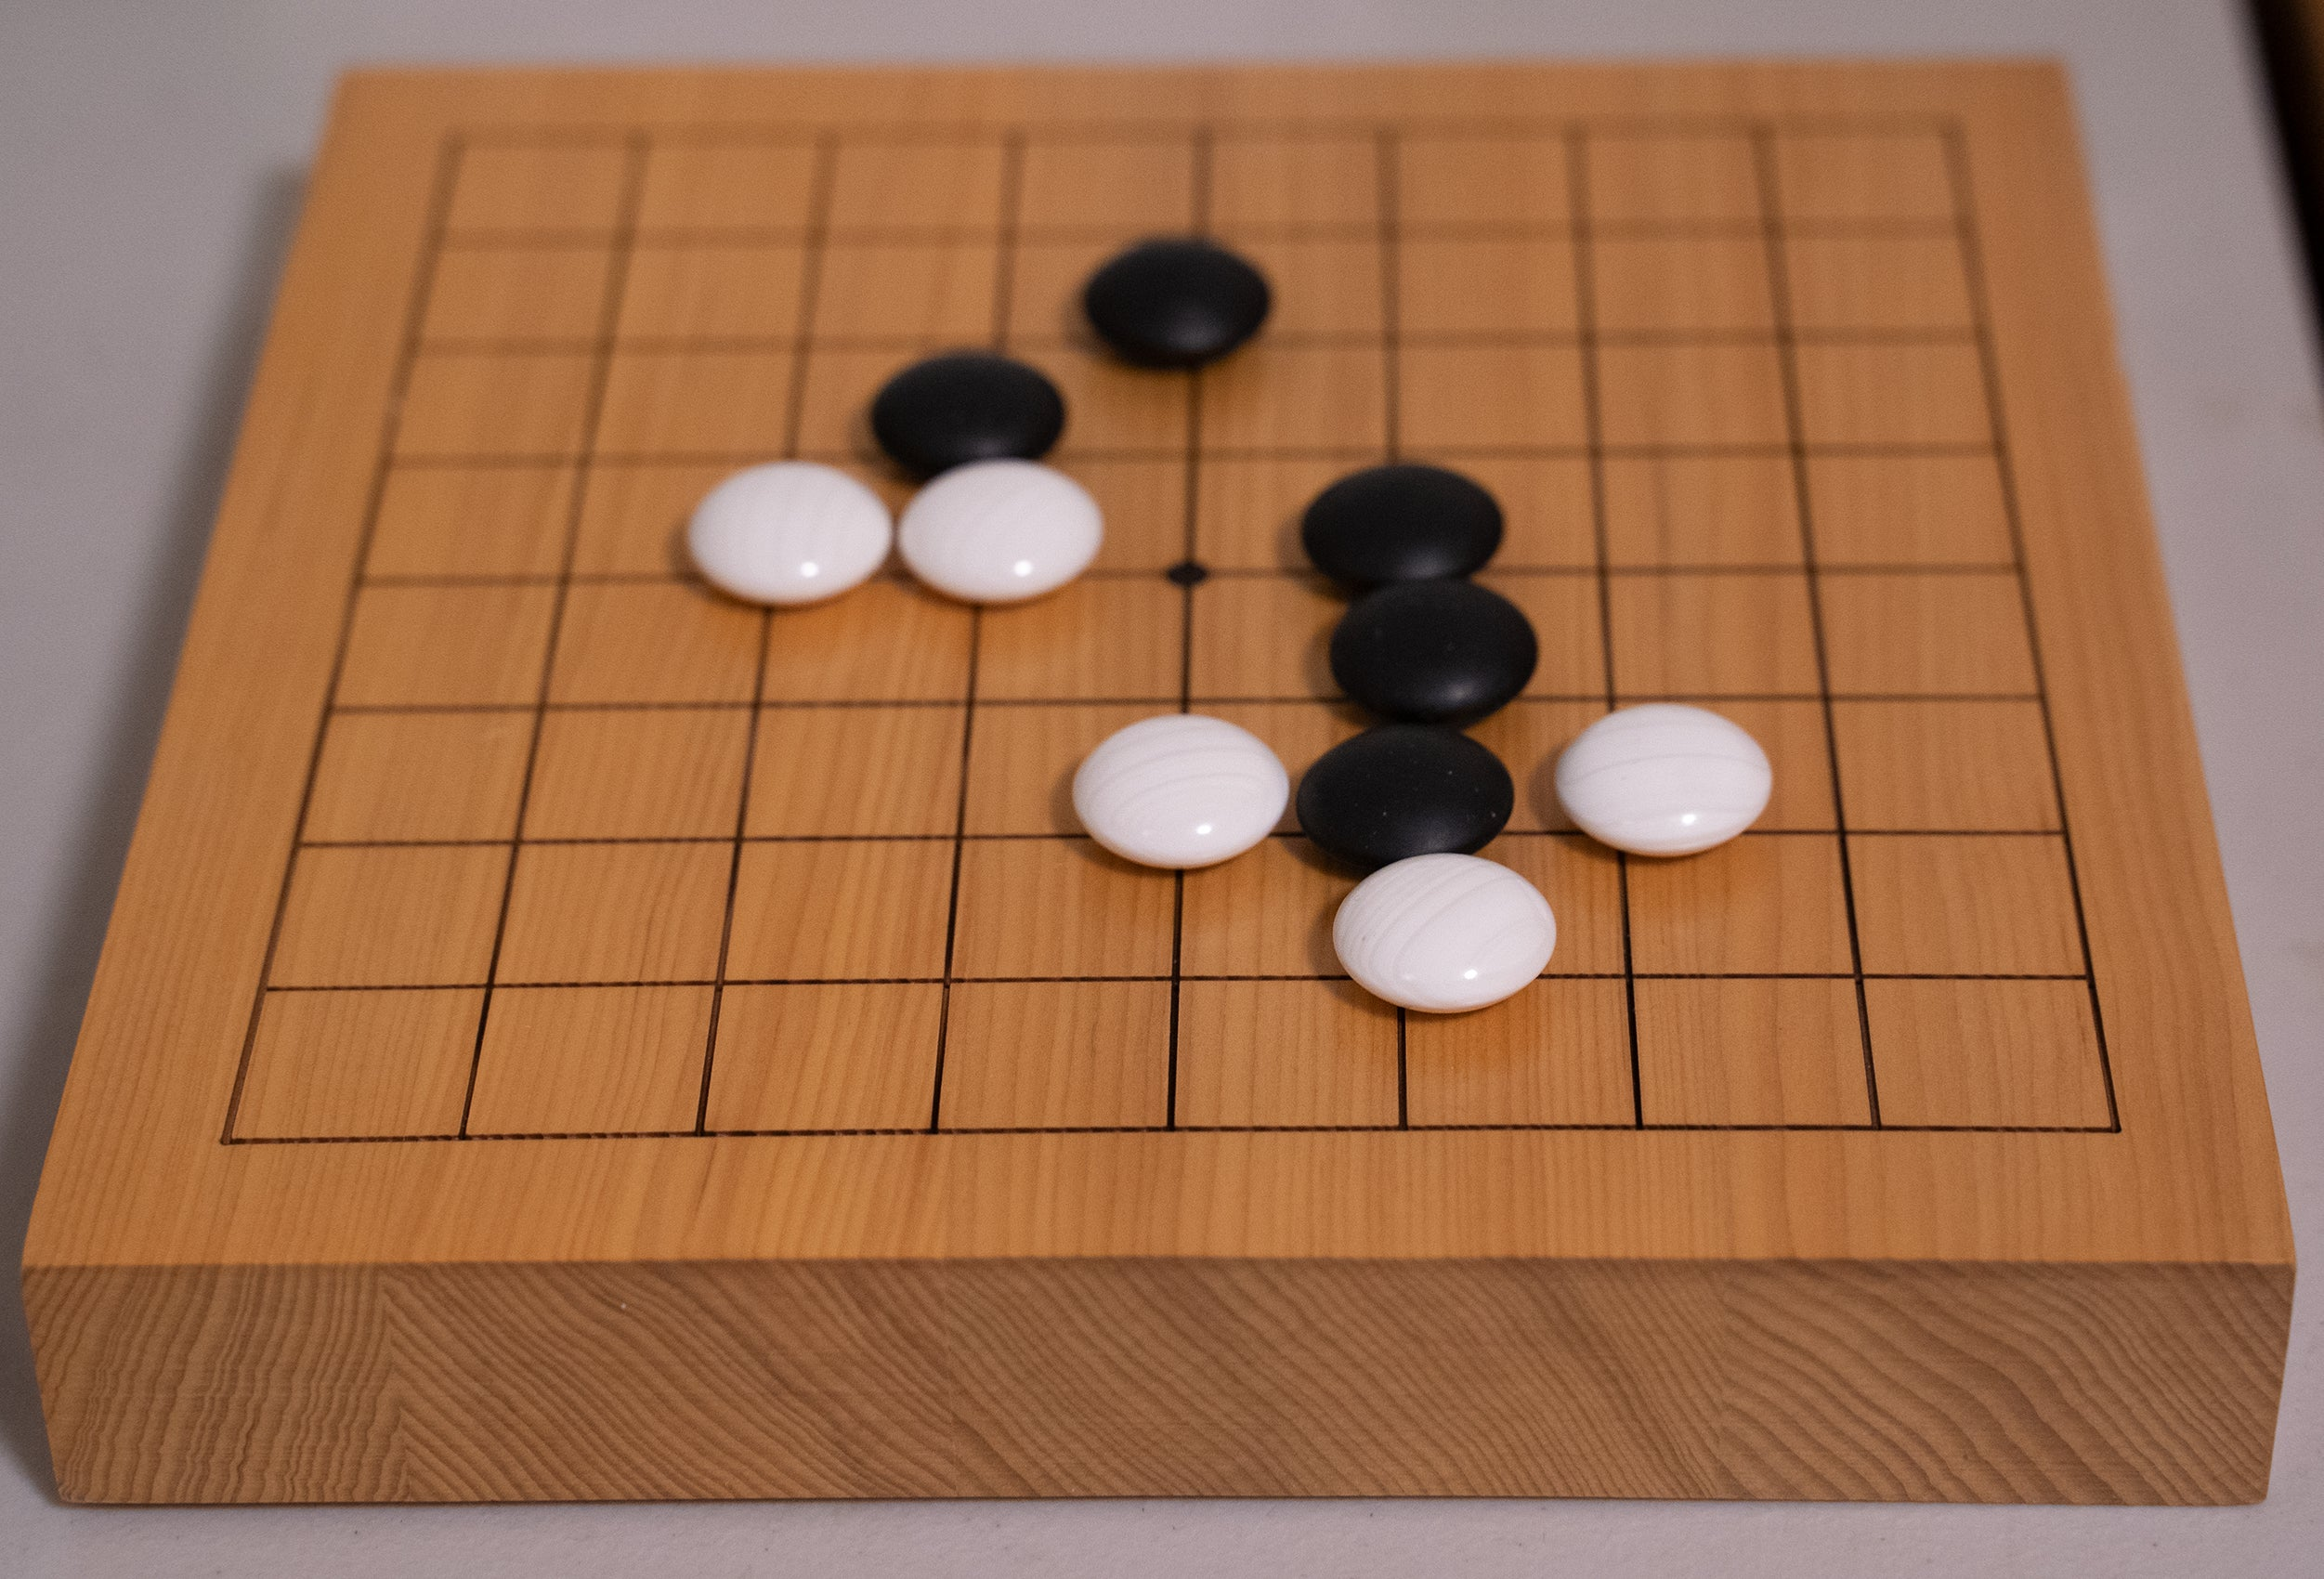
\includegraphics[width=1.0\textwidth]{../tablero.jpg}
\end{figure}
\end{columns}

\end{frame}
%%%%%%%%%%%%%%%%%%%%%%%%%%%%%%%%%%%%%%%%%%%%%%%%%%%%%%%%%%%%%%%%%%%%%%%%%%%%%%%%%%%%%%%%%%%%%%%%%%%%

\begin{frame}
\frametitle{Ventaja y Ranking go}
\begin{columns}
 
\column{.5\textwidth}
 
\textbf{Komi}
\begin{itemize}
 \item Puntos extra al jugador blanco al finalziar la partida
 \item Neutralizar ventaja por iniciar primero
 \item No afecta durante juego
 \item Evitar empate
  \item No hay valor universal
\end{itemize}
\only<1>{\begin{mdframed}[backgroundcolor=frenchblue!0,linecolor=frenchblue!0]
\textbf{Handicap}
\begin{itemize}
 \item Emparejar partida por diferencia de habilidad grande
 \item Fichas negras extra en el inicio de partida
 \item Afecta al juego desde el inicio
\end{itemize}
\end{mdframed}}

\only<2>{\begin{mdframed}[backgroundcolor=frenchblue!20]
\textbf{Handicap}
\begin{itemize}
 \item Emparejar partida por diferencia de habilidad grande
 \item Fichas negras extra en el inicio de partida
  \item Afecta al juego desde el inicio
\end{itemize}
\end{mdframed}}


 \column{.5\textwidth}
 \vspace{-2cm}
\begin{itemize}
 \item Sistema de ranking: 30-1Kyu y 1-9 Dan, principiante a experto
 \item Ficha negra inicializa el juego (jugador mas debil)
 \item 1 piedra de handicap por cada rango de diferencia
\end{itemize}

\vspace{2cm}
\begin{center}
 Servidor KGS
\end{center}



\end{columns}

\end{frame}
%%%%%%%%%%%%%%%%%%%%%%%%%%%%%%%%%%%%%%%%%%%%%%%%%%%%%%%%%%%%%%%%%%%%%%%%%%%%%%%%%%%%%%%%%%%%%%%%%%%%

\begin{frame}
\frametitle{Bayes}

Bayes
\begin{equation*}
p(x,y) = p(x|y) p(y)
\end{equation*}

Volver a ver el video de bishop
\begin{equation*}
\underbrace{p(\overbrace{\text{Skills}}^{Oculto}|\overbrace{\text{Result,Model}}^{Observable})}_{\text{Posterior}} = \frac{\overbrace{P(\text{Result}|\text{Skills,Model})}^{\text{likelihood}}\overbrace{p(\text{Skills})}^{\text{Prior}}}{\underbrace{P(\text{Result}|\text{Model})}_{\text{Evidencia}}}
\end{equation*}

\end{frame}

%%%%%%%%%%%%%%%%%%%%%%%%%%%%%%%%%%%%%%%%%%%%%%%%%%%%%%%%%%%%%%%%%%%%%%%%%%%%%%%%%%%%%%%%%%%%%%%%%%%%


\begin{frame}
\frametitle{Grafico de factores}

\begin{itemize}
 \vspace{0.2cm}\item Dependencias visibles
 \vspace{0.2cm}\item M\'ultiples factorizaciones
\end{itemize}

\begin{equation*}
	f(x,y,z) = (x+y)(y+z)(x+z)
	\end{equation*}
\vspace{-0.2cm}

	\begin{figure}
		\centering
		\begin{subfigure}{0.55\textwidth}
			\centering
            \resizebox{0.65\columnwidth}{!}{%
                \begin{tikzpicture}
				\node[latent] (s1) {$x$} ; %
				\node[factor, below=of s1,xshift=-1.4cm] (fp0) {} ;
				\node[const, left=of fp0] (fp0a) {$(x+y)$}; %
				\node[factor, below=of s1,xshift=1.4cm] (fp2) {} ;
				\node[const, right=of fp2] (fp2a) {$(x+z)$}; %


				\node[latent, below=of fp0,xshift=-.4cm] (p0) {$y$} ; %
				\node[latent, below=of fp2,xshift=.4cm] (p2) {$z$} ; %
				\node[factor, right=of p0, below=of s1, yshift=-1.6cm] (fp1) {} ;
				\node[const, below=of fp1] (fp1a) {$(y+z)$}; %
				
				\edge[-] {s1} {fp0,fp2};
				\edge[-] {fp0} {p0};
				\edge[-] {fp2} {p2};
				\edge[-] {p0} {fp1};
				\edge[-] {fp1} {p2};
            \end{tikzpicture}
			}
		\end{subfigure}%
		\begin{subfigure}{0.55\textwidth}
			\centering
			\resizebox{0.65\columnwidth}{!}{%
                \begin{tikzpicture}
				\node[latent] (s1) {$x$} ; %
				\node[factor, below=of s1] (fp0) {} ;
				\node[const, right=of fp0] (fp0a) {$ (x+y)(y+z)(x+z)$}; %

				\node[latent, below=of fp0,xshift=-1.4cm] (p0) {$y$} ; %
				\node[latent, below=of fp0,xshift=1.4cm] (p2) {$z$} ; %

				\edge[-] {s1} {fp0};
				\edge[-] {p0} {fp0};
				\edge[-] {p2} {fp0};
				\end{tikzpicture}
			}
		\end{subfigure}
	\end{figure}

\end{frame}


%%%%%%%%%%%%%%%%%%%%%%%%%%%%%%%%%%%%%%%%%%%%%%%%%%%%%%%%%%%%%%%%%%%%%%%%%%%%%%%%%%%%%%%%%%%%%%%%%%%%

\begin{frame}
 \frametitle{Grafico de factores}
 \begin{itemize}
 \vspace{0.2cm}\item Marginalizar variable de interes
 \vspace{0.2cm}\item Aprovechar factorizacion $\rightarrow$ pasaje de mensajes
\end{itemize}
vmensaje  f2 a w y x a f2 son dependientes.....
\vspace{-1cm}
\begin{figure}[H]
	\centering
	\tikz{ %
        \node[latent, xshift=-5cm] (v) {$v$} ; %
        \node[factor, right=of v] (f1) {} ;
		\node[const, below=of f1] (nf1) {$f_{1}(v,w)$}; %
		\only<1>{\node[latent, right=of f1] (w) {$w$} ;} %
        \only<2,3,4>{\node[latent, right=of f1, fill=cyan!50] (w) {$w$} ; }%
        
        \node[factor, right=of w] (f2) {} ;
		\node[const, below=of f2] (nf2) {$f_{2}(w,x)$}; %
		\node[latent, right=of f2] (x) {$x$} ; %

        \node[factor, right=of x,yshift=1cm] (f3) {} ;
		\node[const, above=of f3] (nf3) {$f_{3}(x,y)$}; %
		\node[latent, right=of f3] (y) {$y$} ; %
		
        \node[factor, right=of x,yshift=-1cm] (f4) {} ;
		\node[const, below=of f4] (nf4) {$f_{4}(x,z)$}; %
		\node[latent, right=of f4] (z) {$z$} ; %

        \edge[-] {v} {f1}
        \edge[-] {w} {f1,f2}
        \edge[-] {x} {f2,f3,f4}
        \edge[-] {z} {f4}
        \edge[-] {y} {f3}
        \pause
        
        \draw[->,, transform canvas={yshift=0.25cm},color=red!] (f1) -- (w) node[midway,above=3pt,color=red!] {\scriptsize $m_{f_1 \rightarrow w}$} (w);
        \draw[->,, transform canvas={yshift=0.25cm},color=red!] (f2) -- (w) node[midway,above=3pt,color=red!] {\scriptsize $m_{f_2 \rightarrow w}$} (w); \pause

        \draw[->,, transform canvas={yshift=0.25cm},color=red!] (x) -- (f2) node[midway,above=3pt,color=red!] {\scriptsize $m_{x \rightarrow f_2}$} (x); \pause
        
        
        \draw[->,, transform canvas={yshift=0.25cm},color=red!] (f3) -- (x) node[midway,above=2pt,color=red!, rotate=35] {\scriptsize $m_{f_3 \rightarrow x}$} (f3);
        \draw[->,, transform canvas={yshift=-0.25cm},color=red!] (f4) -- (x) node[midway,below=2pt,color=red!, rotate=-30] {\scriptsize $m_{f_4 \rightarrow x}$} (f4); 

        

    
	}
\end{figure}


\begin{equation*}
  \only<1>{p(w) = \sum_v \sum_x \sum_y \sum_z f_1(v,w)f_2(w,x)f_3(x,y)f_4(x,z)}
  %
  \only<2>{p(w) = \underbrace{\left[\sum_v f_1(v,w) \right]}_{m_{f_1 \rightarrow w}} \cdot \underbrace{\left[\sum_x \sum_y \sum_z f_2(w,x)f_3(x,y)f_4(x,z)\right]}_{m_{f_2 \rightarrow w}} }
  %
  \only<3>{p(w) = \underbrace{\left[\sum_v f_1(v,w) \right]}_{m_{f_1 \rightarrow w}}\cdot \underbrace{\left[\sum_x f_2(w,x) \right]}_{m_{f_2 \rightarrow w}}\cdot\underbrace{\left[\sum_y \sum_z f_3(x,y)f_4(x,z)\right] }_{m_{x \rightarrow f_2}}}
  %
  \only<4>{p(w) = \underbrace{\left[\sum_v f_1(v,w) \right]}_{m_{f_1 \rightarrow w}}\cdot \Big[\sum_x f_2(w,x) \underbrace{\left(\sum_y  f_3(x,y)\right)}_{m_{f_3 \rightarrow x}}\underbrace{\left(\sum_zf_4(x,z)\right) }_{m_{f_4 \rightarrow x}}\Big]}
\end{equation*}

\end{frame}
%%%%%%%%%%%%%%%%%%%%%%%%%%%%%%%%%%%%%%%%%%%%%%%%%%%%%%%%%%%%%%%%%%%%%%%%%%%%%%%%%%%%%%%%%%%%%%%%%%%%

\section{Modelos}

\begin{frame}
\frametitle{TrueSkill-\'unico evento}
Quizas menos de mensajes y mas de como es el modelo trueskill antes de mostrar el grafico y demas...

\begin{columns}
\column{0.5\textwidth}
\begin{itemize}
 \item Habilidad gaussiana $\sim \mathcal{N}(s|\mu,\sigma^2)$.
 \item Rendimiento gaussiano, desempe\~no en un dado evento $\sim \mathcal{N}(p|\mu,\beta^2)$.
 \item Rendimiento equipo = suma de rendimientos de integrantes.
 \item Jugador/equipo con mayor rendimiento es el ganador.
 \item Jugadores nuevos inician con mismo $\mu_0$ y $\sigma_0$.
 \item Mismo $\beta$ en todos los eventos y jugadores.
\end{itemize}

% \begin{figure}[H]
% 	\centering
% 	\includegraphics[width=1.0\textwidth]{gaussian.pdf}
% \end{figure}

\column{0.5\textwidth}
    \begin{figure}
        \centering
            \resizebox{0.8\columnwidth}{!}{%
                \begin{tikzpicture}
                % Ejemplo
                        \node[factor] (fs1) {} ;
                        \node[const, right=of fs1] (nfs1) {$f_{s_1}$}; %
                        \node[latent, below=of fs1,yshift=-0.5cm] (s1) {$s_1$} ;

                        \node[factor,below=of s1] (fp1) {} ;
                        \node[const, right=of fp1] (nfp1) {$f_{p_1}$}; %
                        \node[latent, below=of fp1,yshift=-0.5cm] (p1) {$p_1$} ;

                        \node[factor, below= of p1] (fta) {} ;
                        \node[const, right=of fta] (nfta) {$f_{t_a}$}; %
                        \node[latent, below=of fta,yshift=-0.5cm] (ta) {$t_a$} ; %

                        \node[factor, xshift=4cm] (fs2) {} ;
                        \node[const, right=of fs2] (nfs2) {$f_{s_2}$}; %
                        \only<1>{\node[latent, below=of fs2,yshift=-0.5cm] (s2) {$s_2$} ;}
                        \only<2>{\node[latent, below=of fs2,yshift=-0.5cm,fill=cyan!50] (s2) {$s_2$} ;}
                        
                        \node[const, left=of fs2, xshift=5cm] (nfsx) {$f_{s_i}=\mathcal{N}(s_i;\mu_i,\sigma^2)$};

                        \node[factor,below=of s2] (fp2) {} ;
                        \node[const, right=of fp2] (nfp2) {$f_{p_2}$}; %
                        \node[latent, below=of fp2,yshift=-0.5cm] (p2) {$p_2$} ;
                        \node[const, left=of fp2, xshift=5cm] (nfpx) {$f_{p_i}=\mathcal{N}(p_i;s_i,\beta^2)$};

                        \node[factor,below=of p2] (ftb) {} ;
                        \node[const, right=of ftb] (nftb) {$f_{t_b}$}; %
                        \node[const, left=of ftb, xshift=6cm] (nftx) {$f_{t_e}=I(t_e=\sum_{i\in A_e}p_i)$};
                        \node[latent, below=of ftb,yshift=-0.5cm] (tb) {$t_b$} ;

                        \node[factor, below=of tb, xshift=-2cm] (fd) {} ;
                        \node[const, left=of fd] (nfd1) {$f_{d}$}; %
                        \node[const, left=of fd, xshift=6.3cm] (nfdx) {$f_d=I(d_k=t_k-t_{k+1})$};
                        \node[latent, below=of fd,yshift=-0.5cm] (d) {$d$} ; %
                        \node[factor, below=of d,yshift=-0.5cm] (fr) {} ;
                        \node[const, below=of fr] (nfr) {$f_r$}; %
                        \node[const, left=of fr, xshift=5cm] (nfrx) {$f_r=I(d_k>0)$}; %
                        \node[latent, left=of fr, fill=red!50] (r) {$r$} ; %


                        \edge[-] {s1} {fs1,fp1}
                        \edge[-] {s2} {fs2,fp2}
                        \edge[-] {p1} {fp1,fta}
                        \edge[-] {p2} {fp2,ftb}
               


                        \edge[-] {ta} {fta,fd}
                        \edge[-] {tb} {ftb,fd}
                        \edge[-] {d} {fd,fr}
                        \edge[-] {r} {fr}
                        
 

                \end{tikzpicture}
            }
    \end{figure}
\end{columns}

\end{frame}
%%%%%%%%%%%%%%%%%%%%%%%%%%%%%%%%%%%%%%%%%%%%%%%%%%%%%%%%%%%%%%%%%%%%%%%%%%%%%%%%%%%%%%%%%%%%%%%%%%%%


\begin{frame}
\frametitle{Visualizacion}

\begin{columns}
 \column{.5\textwidth}
 \begin{itemize}
 \item Grandes actualizaciones.
\end{itemize}

  \begin{figure}[H]
	\centering
	\only<1>{\includegraphics[width=1.0\textwidth]{trueskill_ej_black_win_prior.pdf}}
	\only<2,3,4>{\includegraphics[width=1.0\textwidth]{trueskill_ej_black_win.pdf}}

\end{figure}
\only<2,3,4>{
 \begin{center}
 Ganador jugador negro
\end{center}
}
 \column{.5\textwidth}
 
  \begin{figure}[H]
	\centering
    \only<3>{\includegraphics[width=1.0\textwidth]{trueskill_ej_black_lose_prior.pdf}}
	\only<4>{\includegraphics[width=1.0\textwidth]{trueskill_ej_black_lose.pdf}}
\end{figure}
\only<3,4>{
\begin{center}
 Ganador jugador blanco
\end{center}}


\end{columns}

\end{frame}
%%%%%%%%%%%%%%%%%%%%%%%%%%%%%%%%%%%%%%%%%%%%%%%%%%%%%%%%%%%%%%%%%%%%%%%%%%%%%%%%%%%%%%%%%%%%%%%%%%%%

\begin{frame}
\frametitle{TrueSkill-M\'ultiples eventos}

que se entienda que el beta es lo que define la escala relativa
\begin{columns}


 \column{.5\textwidth}
 \only<1>{
 \begin{itemize}
 \item La informaci\'on actualizada de un evento se utiliza como prior del pr\'oximo
\end{itemize}


\begin{equation*}
 \underbrace{\mathcal{N}(s_i|\mu_i,\sigma_i^2)}_{Posterior} \rightarrow  \underbrace{\mathcal{N}(s_i|\mu_i,\sigma_i^2)}_{Prior}
\end{equation*}}
\only<2,3>{
 \begin{itemize}
 \item Los jugadores var\'ian su habilidad en el tiempo (mejoran o empeoran)
 \item Problema: Suponer \'unica habilidad por agente.
 \item Soluci\'on: Agregar ruido a la varianza de habilidad.
\end{itemize}


\begin{equation*}
 \underbrace{\mathcal{N}(s_i|\mu_i,\sigma_i^2)}_{Posterior} \rightarrow  \underbrace{\mathcal{N}(s_i|\mu_i,\sigma_i^2+\gamma^2)}_{Prior}
\end{equation*}}

 \column{.5\textwidth}
 \only<3>{
\begin{itemize}
 \item Posterior de un jugador en un evento es el prior del proximo.
 \item Problema: Posterior y prior con distinta forma funcional.
 \item Soluci\'on: \textit{Expectation Propagation}, aproximar mensaje.
\end{itemize}
  \begin{figure}[H]
	\centering
	\includegraphics[width=.8\textwidth]{../trunc.pdf}
\end{figure}}

Esta fea la figura. Aclarar cual es el mensaje
\end{columns}

\end{frame}
%%%%%%%%%%%%%%%%%%%%%%%%%%%%%%%%%%%%%%%%%%%%%%%%%%%%%%%%%%%%%%%%%%%%%%%%%%%%%%%%%%%%%%%%%%%%%%%%%%%%

\begin{frame}
\frametitle{TrueSkill Through Time}
que se entienda que por cada nuevo evento se corre ``todo '' de nuevo
\begin{itemize}
 \vspace{-0.2cm}\item Propagaci\'on informaci\'on futuro a pasado.
 \vspace{-0.2cm}\item Lotes temporales.
 \vspace{-0.2cm}\item Mejor estimaci\'on.
 \vspace{-0.2cm}\item Menor cantidad de partidas necesarios por jugador.
\end{itemize}

\begin{figure}
    \centering
        \resizebox{0.8\columnwidth}{!}{%
            \begin{tikzpicture}
                \node[latent] (s0) {$s_i^{t-1}$} ; %
                \node[factor, below=of s0,yshift=-1cm] (fp01) {} ;
                \node[const, right=of fp01] (nfp01) {$f_{p_i^{t-1}(1)}$}; %
                \node[latent, below=of fp01] (p01) {\footnotesize$p_i^{t-1}(1)$} ; %

                \node[factor, right=of s0,xshift=1cm ] (fs1) {} ;
                \node[const, above=of fs1] (nfs1) {$f_{s_i^{t}}$}; %

                \node[latent, right=of fs1, xshift=1.25cm] (s1) {$s_i^t$} ; %

                \node[factor, right=of s1, xshift=1.25cm ] (fs2) {} ;
                \node[const, above=of fs2] (nfs2) {$f_{s_i^{t+1}}$}; %

                \node[latent, right=of fs2,xshift=1cm] (s2) {$s_i^{t+1}$} ; %
                \node[factor, below=of s2,yshift=-1cm] (fp02) {} ;
                \node[const, right=of fp02] (nfp02) {$f_{p_i^{t+1}(1)}$}; %
                \node[latent, below=of fp02] (p02) {\footnotesize$p_i^{t+1}(1)$} ; %

                \node[factor, below=of s1,yshift=-1cm] (fp0) {} ;
                \node[const, right=of fp0] (nfp0) {$f_{p_i^{t}(1)}$}; %

                \node[factor, color=white, below=of s1] (fp1) {} ;
                %\node[const, right=of fp1] (nfp1) {$f_{p_i^{t}(2)}$}; %



                \node[latent, below=of fp0] (p0) {\footnotesize$p_i^{t}(1)$} ; %



                \edge[-] {s1} {fp0,fp1};
                \edge[-] {fp0} {p0};
                %\edge[-] {fp1} {p1};
                \edge[-] {fp01} {s0,p01}
                \edge[-] {fp02} {s2,p02}
                \edge[-] {fs1} {s0,s1};
                \edge[-] {fs2} {s1,s2};
                %\edge[bend right] {s0} {fs1};
                \path[draw, -latex, fill=black!50] (s0) edge[bend right,draw=black!50] node[midway,below,color=black!75] {\scriptsize \emph{posterior}$(t-1)$} (fs1);
                \path[draw, -latex, fill=black!50] (fs1) edge[bend left,draw=black!50] node[midway,above,color=black!75] {\scriptsize \emph{prior}$(t)$} (s1);
                \path[draw, -latex, fill=black!50] (s2) edge[bend left,draw=black!50] node[midway,below,color=black!75] {\scriptsize \emph{\ \ inversePosterior}$(t+1)$} (fs2);
                \path[draw, -latex, fill=black!50] (fs2) edge[bend right,draw=black!50] node[midway,above,color=black!75] {\scriptsize \emph{inversePrior}$(t)$} (s1);
                \path[draw, -latex, fill=black!50,sloped] (fp0) edge[bend left,draw=black!50] node[midway,below,color=black!75, rotate=90,xshift=-1cm] {\scriptsize \emph{likelihood}$(t,k)$} (s1);
                \path[draw, -latex, fill=black!50,sloped] (s1) edge[bend left,draw=black!50] node[midway,below,color=black!75, rotate=-90,xshift=1cm] {\scriptsize \emph{\ \ withinPrior}$(t,k)$} (fp0);
            \end{tikzpicture}
        }
\end{figure}
\end{frame}
%%%%%%%%%%%%%%%%%%%%%%%%%%%%%%%%%%%%%%%%%%%%%%%%%%%%%%%%%%%%%%%%%%%%%%%%%%%%%%%%%%%%%%%%%%%%%%%%%%%%

\begin{frame}
\frametitle{Metodolog\'ia de evaluaci\'on}
Conteo de microestados?

la productoria tiende a cero, por eso log
\begin{itemize}
 \vspace{-0.2cm}\item Probabilidad de que suceda el observables dadas nuestras hip\'otesis.
 \vspace{-0.2cm}\item Multiplicaci\\'on de las probabilidades todos los eventos.
 \vspace{-0.2cm}\item Logaritmo, productoria $\rightarrow$ suma, penaliza las probabilidades bajas.
 \vspace{-0.2cm}\item Mientras mas cercano a cero, mas certero el modelo.
\end{itemize}

\begin{equation*}
 \text{Evidencia} = -\frac{log(\prod_i^N prob_i)}{N}
\end{equation*}

\end{frame}
%%%%%%%%%%%%%%%%%%%%%%%%%%%%%%%%%%%%%%%%%%%%%%%%%%%%%%%%%%%%%%%%%%%%%%%%%%%%%%%%%%%%%%%%%%%%%%%%%%%%
\section{Validaci\'on}
\begin{frame}
\frametitle{?}

\begin{columns}
 \column{.5\textwidth}
 
 \begin{itemize}
\item Simulacion, dos jugadores.
\item Cambio en el porcentaje de victorias de uno de los jugadores.
 \item Similar probabilidad de victoria estimada y fracci\'on de la misma.
\item Aumento de la misma informaci\'on, aumento de la predicci\'on
\end{itemize}

\begin{equation*}
    \text{lim}_{\text{inf}\rightarrow \infty} \text{Estimaci\'on} = \text{exacta}
\end{equation*}

 
 \column{.5\textwidth}
  \begin{figure}[H]
	\centering
	\includegraphics[width=1.0\textwidth]{synthetic_validation_model_limit.pdf}
\end{figure}
\end{columns}

\end{frame}
%%%%%%%%%%%%%%%%%%%%%%%%%%%%%%%%%%%%%%%%%%%%%%%%%%%%%%%%%%%%%%%%%%%%%%%%%%%%%%%%%%%%%%%%%%%%%%%%%%%%

\begin{frame}
\frametitle{Simulaci\'on: Habilidad conocida}
TrueSkill sale gratis con TTT
\begin{itemize}
 \vspace{-0.2cm}\item Comunidad infinita, \'unico jugador, habilidad conocida.
 \vspace{-0.2cm}\item $\gamma$ ideal en m\'inimo de Evidencia, cercanas entre \texttt{TrueSkill} y \texttt{TTT}.
 \vspace{-0.2cm}\item $\gamma$ bajo, no relaja lo suficiente, incapaz de seguir cambios en habilidad.
  \vspace{-0.2cm}\item $\gamma$ alto, oscilaciones al seguir los cambios en habilidad.
\end{itemize}
\begin{columns}
 \column{.5\textwidth}

  \begin{figure}[H]
	\centering
	\includegraphics[width=1.0\textwidth]{synthetic_validation_gamma_evidencia2.pdf}
\end{figure}
 
 \column{.5\textwidth}
  \only<2>{\begin{figure}[H]
	\centering
	\includegraphics[width=1.0\textwidth]{synthetic_validation_lc_evidencia2.pdf}
\end{figure}}
\end{columns}


\end{frame}

%%%%%%%%%%%%%%%%%%%%%%%%%%%%%%%%%%%%%%%%%%%%%%%%%%%%%%%%%%%%%%%%%%%%%%%%%%%%%%%%%%%%%%%%%%%%%%%%%%%%

\begin{frame}
\frametitle{Par\'ametro $\mu_0$ inicial}

\begin{columns}
\column{0.5\textwidth}
\begin{minipage}[c][0.4\textheight][c]{\linewidth}
  \centering
  \includegraphics[width=0.8\linewidth]{synthetic_model_mu_jugador0.pdf}
\end{minipage}
\begin{minipage}[c][0.4\textheight][c]{\linewidth}
  \centering
  \includegraphics[width=0.8\linewidth]{synthetic_model_mu_jugador12_5.pdf}
\end{minipage}
\column{0.5\textwidth}
\begin{minipage}[c][0.4\textheight][c]{\linewidth}
  \begin{itemize}
  \item Distintos valores de media inicial. 
  \item Los demas parametros iguales.
  \item Misma forma funcional.
  \item Misma probabilidad de ganar
  \item Misma escala relativa
  \end{itemize}
\end{minipage}
\begin{minipage}[c][0.4\textheight][c]{\linewidth}
  \centering
  \includegraphics[width=0.8\linewidth]{synthetic_model_mu_jugador25.pdf}
\end{minipage}
\end{columns}
\end{frame}

%%%%%%%%%%%%%%%%%%%%%%%%%%%%%%%%%%%%%%%%%%%%%%%%%%%%%%%%%%%%%%%%%%%%%%%%%%%%%%%%%%%%%%%%%%%%%%%%%%%%

\begin{frame}
\frametitle{Par\'ametro $\sigma_0$ inicial}

\begin{columns}
 \column{.5\textwidth}
   \begin{itemize}
    \item $\beta$=1 y $\mu_0$=25 fijos.
\item \texttt{TTT} menos sensible al $\sigma_0$.
  \end{itemize}
 
  \begin{figure}[H]
	\centering
	\includegraphics[width=1.0\textwidth]{synthetic_model_sigma_ev.pdf}
\end{figure}
 
 \column{.5\textwidth}
   \begin{itemize}
\item $\beta$=1, $\mu_0$=25 y $\gamma$=1.2 fijos.
  \item \texttt{TTT} converge mas rapido
  \end{itemize}
 
  \begin{figure}[H]
	\centering
	\includegraphics[width=1.0\textwidth]{synthetic_model_sigma_sin_cambios.pdf}
\end{figure}
\end{columns}

\end{frame}
%%%%%%%%%%%%%%%%%%%%%%%%%%%%%%%%%%%%%%%%%%%%%%%%%%%%%%%%%%%%%%%%%%%%%%%%%%%%%%%%%%%%%%%%%%%%%%%%%%%%

\begin{frame}
\frametitle{Par\'ametro $\beta$}

\begin{columns}
 \column{.5\textwidth}
 
  \begin{itemize}
  \item Distintos valores de beta. 
  \item Se mantiene una misma relaci\'on con el $\sigma_0$ ($\sigma_0=3\beta$).
  \item Misma forma funcional.
  \item Misma probabilidad de ganar
  \item Cambio en escala relativa.
  \item Misma escala en t\'erminos de $\beta$.
  \end{itemize}
 
 \column{.5\textwidth}
  \begin{figure}[H]
	\centering
	\includegraphics[width=1.0\textwidth]{synthetic_model_beta_lc.pdf}
\end{figure}
\end{columns}

\end{frame}
%%%%%%%%%%%%%%%%%%%%%%%%%%%%%%%%%%%%%%%%%%%%%%%%%%%%%%%%%%%%%%%%%%%%%%%%%%%%%%%%%%%%%%%%%%%%%%%%%%%%

\section{Resultados}
\begin{frame}
\frametitle{KGS-Datos}

\begin{columns}
\column{0.5\textwidth}
\begin{minipage}[c][0.4\textheight][c]{\linewidth}
  \centering
  \includegraphics[width=0.8\linewidth]{data_date.pdf}
\end{minipage}
\begin{minipage}[c][0.4\textheight][c]{\linewidth}
    \begin{itemize}
     \item 2M partidas, 60k jugadores.
     \item Se filtraron los BOTs y partidas anomalas, 1.6M.
     \item Partidas desde 2007 hasta abril 2019.
     \item Partidas de Danes (restricci\'on de 4to Dan).
    \end{itemize}

\end{minipage}
\column{0.5\textwidth}
\begin{minipage}[c][0.4\textheight][c]{\linewidth}
  \centering
  \includegraphics[width=0.8\linewidth]{lc_rank_hist_blue.pdf}
\end{minipage}
\begin{minipage}[c][0.4\textheight][c]{\linewidth}
  \centering
  \includegraphics[width=0.8\linewidth]{data_handicap.pdf}
\end{minipage}
\end{columns}

\end{frame}
%%%%%%%%%%%%%%%%%%%%%%%%%%%%%%%%%%%%%%%%%%%%%%%%%%%%%%%%%%%%%%%%%%%%%%%%%%%%%%%%%%%%%%%%%%%%%%%%%%%%

\begin{frame}
\frametitle{Modelo handicap}
\begin{columns}
 \column{.5\textwidth}
    \begin{itemize}
     \item \emph{Handicap} como jugador, equipo negro.
     \item Habilidad \'unica $\rightarrow$ $\gamma=0$.
     \item Rendimiento \'unico $\rightarrow$ $\beta=0$.
     \item Jugador distinto por valor de \emph{Handicap}.
    \end{itemize}

 \column{.5\textwidth}
    \begin{figure}
        \centering
            \resizebox{0.8\columnwidth}{!}{%
                \begin{tikzpicture}
                % Ejemplo
                        \node[factor] (fs1) {} ;
                        \node[const, right=of fs1] (nfs1) {$f_{s_1}$}; %
                        \node[latent, below=of fs1,yshift=-0.5cm] (s1) {$s_1$} ;

                        \node[factor,below=of s1] (fp1) {} ;
                        \node[const, right=of fp1] (nfp1) {$f_{p_1}$}; %
                        \node[latent, below=of fp1,yshift=-0.5cm] (p1) {$p_1$} ;

                        \node[factor, below= of p1] (fta) {} ;
                        \node[const, right=of fta] (nfta) {$f_{t_a}$}; %
                        \node[latent, below=of fta,yshift=-0.5cm] (ta) {$t_a$} ; %

                        \node[factor, xshift=3cm] (fs2) {} ;
                        \node[const, right=of fs2] (nfs2) {$f_{s_2}$}; %
                        \node[latent, below=of fs2,yshift=-0.5cm] (s2) {$s_2$} ;
                        
                        \only<2>{\node[factor, xshift=5cm] (fs3) {} ;
                        \node[const, right=of fs3] (nfs3) {$f_{s_3}$}; }
                        \node[const, left=of fs2, xshift=7cm] (nfsx) {$f_{s_i}=\mathcal{N}(s_i;\mu_i,\sigma^2)$};
                        \only<2>{\node[latent, below=of fs3,yshift=-0.5cm] (s3) {$s_3$} ;}

                        \node[factor,below=of s2] (fp2) {} ;
                        \node[const, right=of fp2] (nfp2) {$f_{p_2}$}; %
                        \node[latent, below=of fp2,yshift=-0.5cm] (p2) {$p_2$} ;
                        \only<2>{\node[factor,below=of s3] (fp3) {} ;}
                        \only<2>{\node[const, right=of fp3] (nfp3) {$f_{p_3}$};} %
                        \node[const, left=of fp2, xshift=7cm] (nfpx) {$f_{p_i}=\mathcal{N}(p_i;s_i,\beta^2)$};
                        \only<2>{\node[latent, below=of fp3,yshift=-0.5cm] (p3) {$p_3$} ;}

                        \node[factor,below=of p2, xshift=1cm] (ftb) {} ;
                        \node[const, right=of ftb] (nftb) {$f_{t_b}$}; %
                        \node[const, left=of ftb, xshift=6cm] (nftx) {$f_{t_e}=I(t_e=\sum_{i\in A_e}p_i)$};
                        \node[latent, below=of ftb,yshift=-0.5cm] (tb) {$t_b$} ;

                        \node[factor, below=of tb, xshift=-2cm] (fd) {} ;
                        \node[const, left=of fd] (nfd1) {$f_{d}$}; %
                        \node[const, left=of fd, xshift=6.3cm] (nfdx) {$f_d=I(d_k=t_k-t_{k+1})$};
                        \node[latent, below=of fd,yshift=-0.5cm] (d) {$d$} ; %
                        \node[factor, below=of d,yshift=-0.5cm] (fr) {} ;
                        \node[const, below=of fr] (nfr) {$f_r$}; %
                        \node[const, left=of fr, xshift=5cm] (nfrx) {$f_r=I(d_k>0)$}; %
                        \node[latent, left=of fr, fill=red!50] (r) {$r$} ; %


                        \edge[-] {s1} {fs1,fp1}
                        \edge[-] {s2} {fs2,fp2}
                       \only<2>{ \edge[-] {s3} {fs3,fp3}}
                        \edge[-] {p1} {fp1,fta}
                        \edge[-] {p2} {fp2,ftb}
                       \only<2>{ \edge[-] {p3} {fp3,ftb}}


                        \edge[-] {ta} {fta,fd}
                        \edge[-] {tb} {ftb,fd}
                        \edge[-] {d} {fd,fr}
                        \edge[-] {r} {fr}
                        

                \end{tikzpicture}
            }
    \end{figure}

\end{columns}
\end{frame}
%%%%%%%%%%%%%%%%%%%%%%%%%%%%%%%%%%%%%%%%%%%%%%%%%%%%%%%%%%%%%%%%%%%%%%%%%%%%%%%%%%%%%%%%%%%%%%%%%%%%

\begin{frame}
\frametitle{TTT-Handicap}
SI O SI defender y contar cuanto significa la diferencia entre TTT con handicap y sin
    \begin{itemize}
     \item Revision de parametros.
     \item Mejor evidencia con \texttt{TTT} con \emph{handicap}.
     \item $\gamma=0.0075$, $\sigma_0=3\beta$.
    \end{itemize}
\begin{columns}
\column{.5\textwidth}

       \begin{figure}[H]
        \centering
        \includegraphics[width=.9\textwidth]{rela_beta_sigma.pdf}
    \end{figure}
\column{.5\textwidth}

 
  \begin{figure}[H]
        \centering
        \includegraphics[width=.9\textwidth]{evidence_gamma.pdf}
    \end{figure}
\end{columns}


\end{frame}
%%%%%%%%%%%%%%%%%%%%%%%%%%%%%%%%%%%%%%%%%%%%%%%%%%%%%%%%%%%%%%%%%%%%%%%%%%%%%%%%%%%%%%%%%%%%%%%%%%%%


\begin{frame}
\frametitle{Caracterizaci\'on Handicap}
Tiene que estar la ecuacion de calculo de la probabilidad
    \begin{itemize}
     \vspace{-0.4cm}\item Cambio $\beta$, pendiente uno (escala relativa).
     \vspace{-0.4cm}\item Comportamiento lineal.
    \vspace{-0.4cm} \item H$_9$ caso limite, no se inculye al ajuste.
     \only<3,4>{\vspace{-0.4cm}\item 1000 puntos normalmente distribuidos por \emph{handicap}.}
      \only<4>{\vspace{-0.4cm}\item $84\%$ de las partidas en intervalo de probabilidad de $25-70\%$.}
    \end{itemize}
\begin{columns}
 \column{.5\textwidth}
   \only<1>{ \begin{figure}[H]
	\centering
	\includegraphics[width=1.0\textwidth]{handicap_fit_sinFit.pdf}
\end{figure}
\begin{center}
    $\beta=1$
\end{center}}
  \only<2>{ \begin{figure}[H]
	\centering
	\includegraphics[width=1.0\textwidth]{handicap_fit_uno_sinFit.pdf}
\end{figure}
\begin{center}
     $\beta=1$ vs $\beta=4.45$
\end{center}}
 \only<3,4>{   \begin{figure}[H]
	\centering
	\includegraphics[width=1.0\textwidth]{handicap_fit_uno.pdf}
\end{figure}
\begin{center}
    $\beta=4.45$
\end{center}
}
 
 \column{.5\textwidth}

  \only<4>{\begin{figure}[H]
	\centering
	\includegraphics[width=1.0\textwidth]{probability_H_sigmoide.pdf}
\end{figure}}
\end{columns}
\end{frame}
%%%%%%%%%%%%%%%%%%%%%%%%%%%%%%%%%%%%%%%%%%%%%%%%%%%%%%%%%%%%%%%%%%%%%%%%%%%%%%%%%%%%%%%%%%%%%%%%%%%%


\begin{frame}
\frametitle{Comparaci\'on}
\begin{columns}
 \column{.5\textwidth}
     \begin{itemize}
        \item Partidas separadas en intervalos de probabilidad estimada.
        \item Estimaci\'on vs frecuencia de victorias.
    \end{itemize}
   \begin{figure}[H]
	\centering
	\includegraphics[width=1.0\textwidth]{probability_H_hist_prob_real1.pdf}
\end{figure}
 
 \column{.5\textwidth}
     \begin{itemize}
        \item Utilizaci\'on de valores de handicap que resultan en partidas equiprobables.
        \item Estimaciones hechas con handicap propuesto.
        \item Teoricamente distribucion de menor varianza centrado en el equiprobable.
    \end{itemize}
  \begin{figure}[H]
	\centering
	\includegraphics[width=1.0\textwidth]{probability_H_hist_prob_real2.pdf}
\end{figure}
\end{columns}

\end{frame}
%%%%%%%%%%%%%%%%%%%%%%%%%%%%%%%%%%%%%%%%%%%%%%%%%%%%%%%%%%%%%%%%%%%%%%%%%%%%%%%%%%%%%%%%%%%%%%%%%%%%


\begin{frame}
\frametitle{Handicap asignado}
     \begin{itemize}
     \vspace{-0.4cm}\item Filtros por condicion entre valor handicap propuesto y usado.
     \vspace{-0.4cm}\item Comparacion entre el porcentaje de victorias en cada caso y el equiporbable.
    \end{itemize}
\begin{columns}
 \column{.5\textwidth}
 
   \begin{figure}[H]
	\centering
	\includegraphics[width=1.0\textwidth]{estimations_H_noH.pdf}
\end{figure}
 \begin{center}
   Valor de Handicap utilizado = 1
 \end{center}

 \column{.5\textwidth}
  \begin{figure}[H]
	\centering
	\includegraphics[width=1.0\textwidth]{estimations_H_good.pdf}
\end{figure}
 \begin{center}
   Valor de Handicap utilizado = al handicap propuesto
 \end{center}
\end{columns}

\end{frame}
%%%%%%%%%%%%%%%%%%%%%%%%%%%%%%%%%%%%%%%%%%%%%%%%%%%%%%%%%%%%%%%%%%%%%%%%%%%%%%%%%%%%%%%%%%%%%%%%%%%%


\begin{frame}
\frametitle{Handicap asignado}
\begin{columns}
 \column{.5\textwidth}
 
   \begin{figure}[H]
	\centering
	\includegraphics[width=1.0\textwidth]{estimations_H_less.pdf}
\end{figure}
  \begin{center}
   Valor de Handicap utilizado = por debajo al propuesto
 \end{center}
 \column{.5\textwidth}
  \begin{figure}[H]
	\centering
	\includegraphics[width=1.0\textwidth]{estimations_H_color.pdf}
\end{figure}
 \begin{center}
   Valor de Handicap utilizado = 1
 \end{center}
\end{columns}

\end{frame}
%%%%%%%%%%%%%%%%%%%%%%%%%%%%%%%%%%%%%%%%%%%%%%%%%%%%%%%%%%%%%%%%%%%%%%%%%%%%%%%%%%%%%%%%%%%%%%%%%%%%

\begin{frame}
\frametitle{Estimacion}
\begin{columns}
 \column{.5\textwidth}
     \begin{itemize}
        \item Simulacion en utilizacion online.
        \item 500 partidas seleccionadas \rightarrow base de datos de estudio.
        \item Remanente de partidas \rightarrow base de datos de entrenamiento.
        \item No repetir jugadores.
        \item Condicion jugadores conocidos ($\sigma$ bajo).
        \item Condicion en rango.
        \item Condicion eliminacion de partidas futuras a la seleccionada.
    \end{itemize} 
 
 \column{.5\textwidth}
  \begin{figure}[H]
	\centering
	\includegraphics[width=1.0\textwidth]{study_same_rank.pdf}
\end{figure}
\begin{center}
 Mismo rango.
\end{center}

\end{columns}


\end{frame}
%%%%%%%%%%%%%%%%%%%%%%%%%%%%%%%%%%%%%%%%%%%%%%%%%%%%%%%%%%%%%%%%%%%%%%%%%%%%%%%%%%%%%%%%%%%%%%%%%%%%
\section{Conclusiones}
\begin{frame}
\frametitle{Trabajo a futuro}
     \begin{itemize}
        \item Trabajo similar, modelando el \emph{komi} como jugador en equipo blanco.
        \item Estudio del efecto del tama\~no de los lotes del modelo \texttt{TTT}.
        \item Optimizar y paralelizar el codigo para realizar el estudio en forma online en tiempos de computo razonables.
    \end{itemize} 

\end{frame}
%%%%%%%%%%%%%%%%%%%%%%%%%%%%%%%%%%%%%%%%%%%%%%%%%%%%%%%%%%%%%%%%%%%%%%%%%%%%%%%%%%%%%%%%%%%%%%%%%%%%

\begin{frame}
\frametitle{Conclusiones}
     \begin{itemize}
        \item Estudio y entendimiento del modelo \texttt{TrueSkill} y su sucesor.
        \item Caracterizacion de la habilidad del handicap.
        \item Sistema de ranking juego go.
        \item Mejorar en el sistema de asignacion de handicap.
    \end{itemize} 
\end{frame}
%%%%%%%%%%%%%%%%%%%%%%%%%%%%%%%%%%%%%%%%%%%%%%%%%%%%%%%%%%%%%%%%%%%%%%%%%%%%%%%%%%%%%%%%%%%%%%%%%%%%

\begin{frame}
\frametitle{?}
\begin{columns}
 \column{.3\textwidth}
  \column{.4\textwidth}
\begin{mdframed}[backgroundcolor=frenchblue!20]
\centering
\vspace{0.3cm}
Muchas gracias! \\
\vspace{1cm}
Preguntas?
\vspace{0.3cm}
\end{mdframed}
 \column{.3\textwidth}
\end{columns}
\end{frame}
%%%%%%%%%%%%%%%%%%%%%%%%%%%%%%%%%%%%%%%%%%%%%%%%%%%%%%%%%%%%%%%%%%%%%%%%%%%%%%%%%%%%%%%%%%%%%%%%%%%%
\appendix
\section{Extra}
%%%%%%%%%%%%%%%%%%%%%%%%%%%%%%%%%%%%%%%%%%%%%%%%%%%%%%%%%%%%%%%%%%%%%%%%%%%%%%%%%%%%%%%%%%%%%%%%%%%%

\begin{frame}
\frametitle{Estimacion}

  \begin{figure}[H]
	\centering
	\includegraphics[width=1.0\textwidth]{study_diff_rank.pdf}
\end{figure}
\end{frame}
\end{document}
